\section{Tool Bar}

There is a tool bar for performing various frequently used commands. These are listed below in their order from left to right in the given figure:

\begin{itemize}
\item Back - navigates back to the previous item
\item Forward - navigates forward to the next item
\item Revert - reverts the project back to it's original form
\item Undo - undoes the last change
\item Redo - redoes the last change
\item Add new item - you can specify the type in the drop down
\item Delete current item
\item Save the project
\item Save As
\item Open a new project
\item Generate a report - opens report generation window
\item Send feedback to the developers on bugs
\end{itemize}

\begin{figure}[H]
\centering
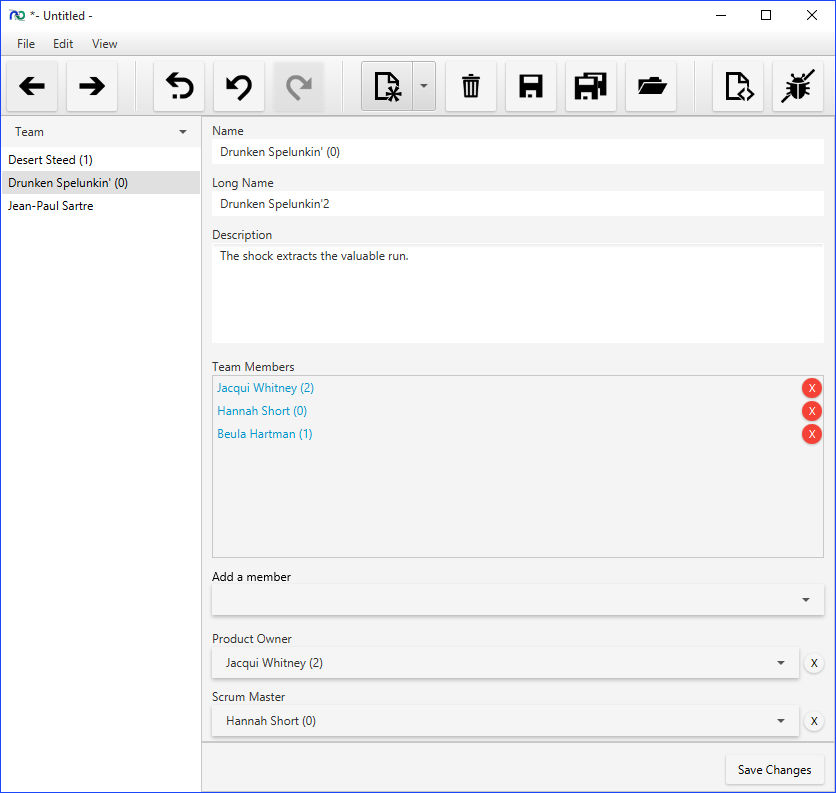
\includegraphics[width=\textwidth]{images/screenshots/toolbar.PNG}
\caption{Tool Bar}
\label{fig:new_project}
\end{figure}

It is also possible to hide sections of the toolbar. In order to do this right click on the toolbar (not on one of the buttons) and a context menu will appear with the sections of the toolbar that you can show and hide, as shown in the figure below.

\begin{figure}[H]
\centering
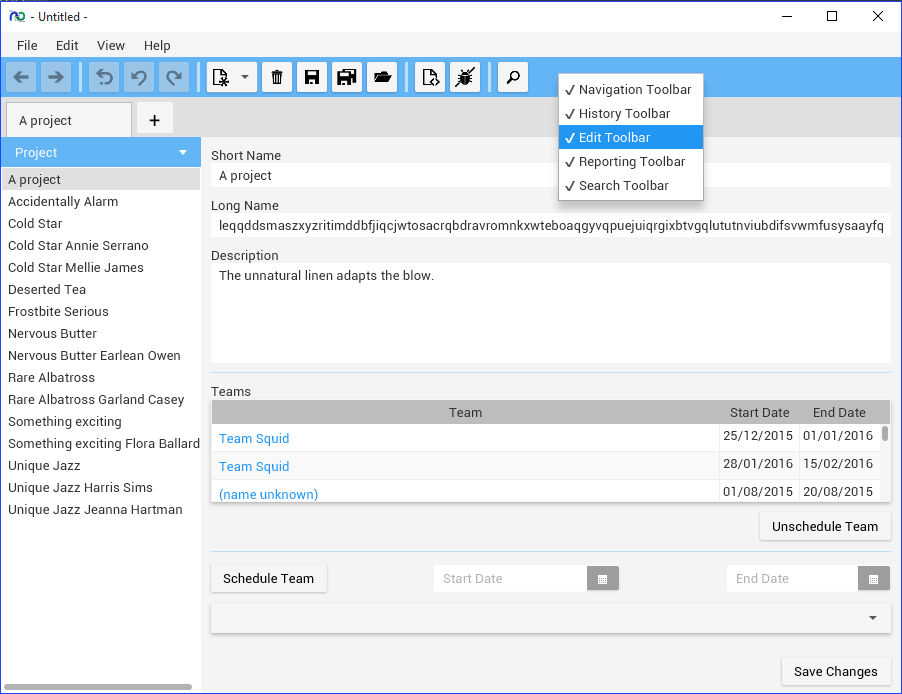
\includegraphics[width=\textwidth]{images/screenshots/toolbar1.PNG}
\caption{The Tool Bar Hides (Because you're scary)}
\label{fig:new_project}
\end{figure}